\usetikzlibrary{positioning}
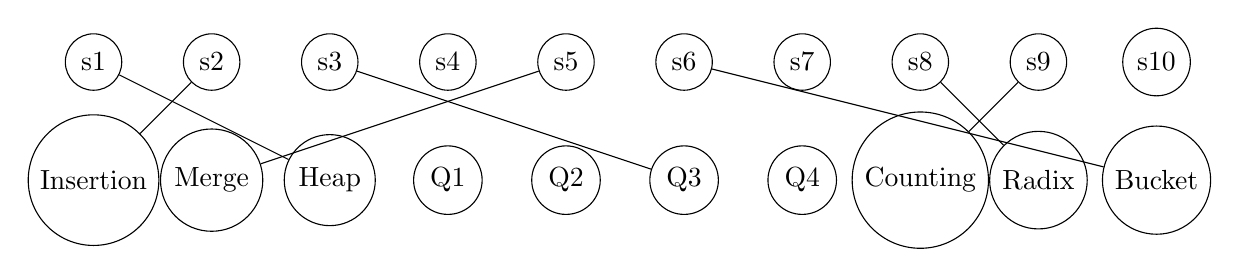
\begin{tikzpicture}[node distance=1.5cm,circle=all,on grid]
 %   \tikzstyle{every node}=[font=\tiny]
 \node[draw] (s1)  at (0:0)	 {s1 };
 \node[draw] (s2)  [right=of s1] {s2 };
 \node[draw] (s3)  [right=of s2] {s3 };
 \node[draw] (s4)  [right=of s3] {s4 };
 \node[draw] (s5)  [right=of s4] {s5 };
 \node[draw] (s6)  [right=of s5] {s6 };
 \node[draw] (s7)  [right=of s6] {s7 };
 \node[draw] (s8)  [right=of s7] {s8 };
 \node[draw] (s9)  [right=of s8] {s9 };
 \node[draw] (s10) [right=of s9] {s10};
 \node[draw] (Insertion)[below=of s1] {Insertion};
 \node[draw] (Merge)	[below=of s2] {Merge	};
 \node[draw] (Heap) 	[below=of s3] {Heap 	};
 \node[draw] (Q1) 	[below=of s4] {Q1 	};
 \node[draw] (Q2) 	[below=of s5] {Q2 	};
 \node[draw] (Q3) 	[below=of s6] {Q3 	};
 \node[draw] (Q4) 	[below=of s7] {Q4 	};
 \node[draw] (Counting) [below=of s8] {Counting	};
 \node[draw] (Radix)	[below=of s9] {Radix	};
 \node[draw] (Bucket)	[below=of s10]{Bucket	};
\path[-]
 (s1) edge (Heap)
 (s2) edge (Insertion)
 (s3) edge (Q3)
 (s5) edge (Merge)
 (s6) edge (Bucket)
 (s8) edge (Radix)
 (s9) edge (Counting)
;
\end{tikzpicture}

